\documentclass[12pt]{article}
\usepackage{fullpage}
\usepackage{graphicx}
\usepackage{color}
\usepackage{amsmath}
\usepackage{amsfonts}
\usepackage{listings}
\usepackage{framed}
\usepackage[pdftex,pdfborder={0 0 0}]{hyperref}

\newcommand{\uo}{\mathrm{UO}_2}
\newcommand{\K}{\ensuremath{\mbox{K}}}
\newcommand{\W}{\ensuremath{\mbox{W}}}
\newcommand{\M}{\ensuremath{\mbox{M}}}
\newcommand{\C}{\ensuremath{\mbox{C}}}
\newcommand{\kg}{\ensuremath{\mbox{kg}}}
\newcommand{\m}{\ensuremath{\mbox{m}}}
\newcommand{\inch}{\ensuremath{\mbox{in}}}
\newcommand{\clad}{\ensuremath{\mbox{clad}}}


%opening
\title{2D Multimaterial Heat Conduction in Cylindrical Geometry With Source}
\author{Glen Hansen}

\begin{document}
\maketitle

\begin{figure}[!htbp]
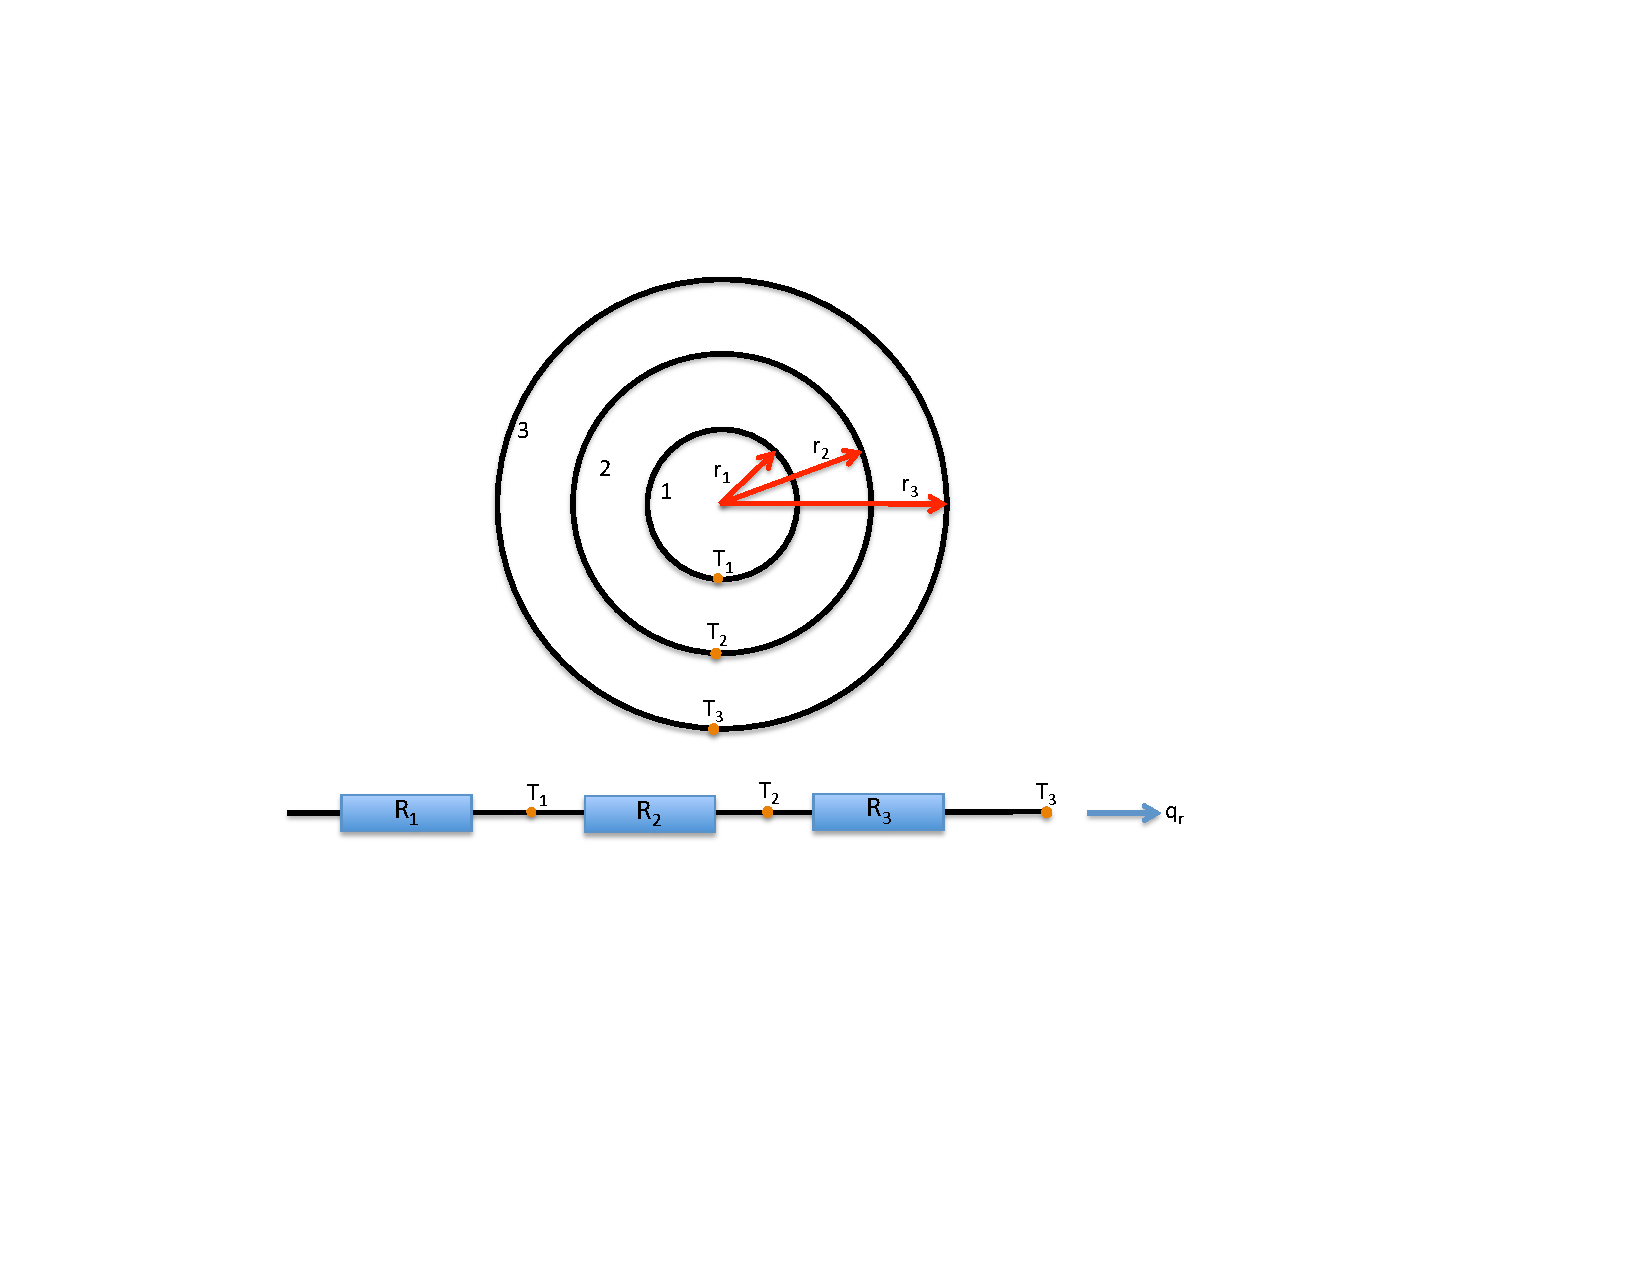
\includegraphics[width=6.5in,trim=100 200 200 100,clip]{cyl}
\caption{Concentric cylindrical model with multiple regions of different thermal conductivity. Region 1 has
conductivity $k_1$, radius $r_1$, internal heat generation term $\dot{q}$, and is made of $\uo$.}
\label{fig:domain}
\end{figure}


This document describes the Albany Heat2DMMCylWithSource test problem. It is a
simple heat conduction problem, with a constant volumetric source in Region~1
(shown in Fig.~\ref{fig:domain}), that is surrounded by two different materials
to form concentric cylinders. Region~1 is meant to be a reactor fuel that
generates heat by radioactive decay at a constant rate $\dot{q}$. A ceramic
material of moderate thermal conductivity $k_1$ and made of $\uo$ fills the
region. The radius is $r_1$, and the outside temperature of this area is $T_1$.

Zircalloy metal, the fuel cladding, surrounds this fuel. The cladding has an outside radius
$r_2$, a conductivity $k_2$, and an outside temperature $T_2$. Lastly, air (or vacuum) surrounds the
cladding. The air region has a thermal conductivity $k_3$, radius $r_3$, and outside temperature $T_3$.
The idea behind this test is to calculate the effective thermal conductivity $k_3$ of the air/vacuum environment
that surrounds the fuel/cladding while it is ``dryed.'' Given a decay heat $\dot{q}$, what is the thermal
conductivity of this material needed such that the peak internal temperature of the fuel (Region~1) does not
exceed $400 C$ given a surrounding environment temperature $T_3$ of $40 C$.

This test is meant to provide a simple steady-state validation of initial capabilities needed to calculate
such things. Here, we model the concentric cylinders in two stages. The first stage uses a simplified form
of (3.28) in
\cite{incropera81}:
%
\begin{equation}
q_r = \frac{T_{\infty,1} - T_{\infty, 4}}{\frac{1}{2\pi r_1 L h_1} + \frac{\ln (r_2 / r_1)}{2\pi k_A L} +
\frac{\ln (r_3 / r_2)}{2 \pi k_B L} + \frac{\ln(r_4/r_3)}{2\pi k_C L} + \frac{1}{2\pi r_4 L h_4}}
\end{equation}

For the problem described in Fig.~\ref{fig:domain}, and assuming that the length of the problem $L$ is
unity, this becomes
%
\begin{equation}
q_r = \frac{T_{1} - T_{3}}{\frac{\ln (r_2 / r_1)}{2\pi k_2} +
\frac{\ln (r_3 / r_2)}{2 \pi k_3} }
\label{eq:resist}
\end{equation}

Now, note that an overall energy balance at a radius of $r_1$ will give
%
\begin{equation}
q_r(r=r_1, \mathrm{inside}) =
q_r(r=r_1, \mathrm{outside}) 
\label{eq:e_balance}
\end{equation}
or
\begin{equation}
\dot{q} (\pi r_1^2) =
\frac{T_{1} - T_{3}}{\frac{\ln (r_2 / r_1)}{2\pi k_2} +
\frac{\ln (r_3 / r_2)}{2 \pi k_3} }
\label{eq:energy_balance}
\end{equation}
or
\begin{equation}
\frac{\dot{q} r_1^2}{2} \left[
\frac{\ln (r_2 / r_1)}{k_2} +
\frac{\ln (r_3 / r_2)}{k_3} \right] =
T_{1} - T_{3}
\end{equation}
or simply
\begin{equation}
\frac{\dot{q} r_1^2}{2} \left[ \quad \cdot \quad \right] =
T_{1} - T_{3}
\label{eq:bal}
\end{equation}

Lastly, note that (3.52) in \cite{incropera81}
%
\begin{equation}
T(r) = \frac{\dot{q} r_o^2}{4 k} \left( 1 - \frac{r^2}{r_o^2}\right) + T_s
\end{equation}
%
may be rewritten for our case of the center cylinder $r_1$ as
%
\begin{equation}
T(r) = \frac{\dot{q}}{4 k_1} \left( r_1^2 - r^2\right) + T_1
\label{eq:fuel_t_1}
\end{equation}

As one is typically most interested in the temperature profile inside the fuel region~1, we can rewrite
\eqref{eq:bal} in terms of $T_1$
%
\begin{equation}
T_{1} =
\frac{\dot{q} r_1^2}{2} \left[ \quad \cdot \quad \right]
+ T_{3}
\end{equation}
%
and substitute this into \eqref{eq:fuel_t_1} to get
%
\begin{equation}
T(r) = \frac{\dot{q}}{4 k_1} \left( r_1^2 - r^2\right) + 
\frac{\dot{q} r_1^2}{2} \left[
\frac{\ln (r_2 / r_1)}{k_2} +
\frac{\ln (r_3 / r_2)}{k_3} \right] + T_3
\label{eq:fuel_t_2}
\end{equation}

To get $T_1$, we evaluate \eqref{eq:fuel_t_2} at $r = r_1$,
%
\begin{equation}
T_1 = \frac{\dot{q} r_1^2}{2} \left[
\frac{\ln (r_2 / r_1)}{k_2} +
\frac{\ln (r_3 / r_2)}{k_3} \right] + T_3.
\label{eq:fuel_t_1a}
\end{equation}

To get $T_2$, we note that $q_r$ in \eqref{eq:e_balance} is constant outside of the fuel $r \leq r_1$, so
\eqref{eq:energy_balance} can be written as:
%
\begin{equation}
\dot{q} (\pi r_1^2) =
\frac{T_{1} - T_{3}}{\frac{\ln (r_2 / r_1)}{2\pi k_2} +
\frac{\ln (r_3 / r_2)}{2 \pi k_3} } =
\frac{T_{2} - T_{3}}{\frac{\ln (r_3 / r_2)}{2 \pi k_3} },
\end{equation}
%
or
%
\begin{equation}
T_2 = \frac{\dot{q} r_1^2}{2} \left[
\frac{\ln (r_3 / r_2)}{k_3} \right] + T_3.
\label{eq:fuel_t_2_a}
\end{equation}

Now, we use (3.25) in \cite{incropera81}, written appropriately, to calculate the
temperature profile in the cladding $r_1 \leq r \leq r_2$,
%
\begin{equation}
T(r) = \frac{T_1 - T_2}{\ln(r_1/r_2)} \ln(\frac{r}{r_2}) + T_2,
\label{eq:T_outer_a}
\end{equation}
%
and again for the cask environment $r_2 \leq r \leq r_3$,
%
\begin{equation}
T(r) = \frac{T_2 - T_3}{\ln(r_2/r_3)} \ln(\frac{r}{r_3}) + T_3.
\label{eq:T_outer_b}
\end{equation}

\section{Use Case}

Here, we will vary $r$ in \eqref{eq:fuel_t_2} to see the temperature variation in region 1, the $\uo$ fuel area. 
The test case for this code is to compare long-time transient results in this region to this steady derivation.

\section{Test Problem}

The test problem in this directory is a single nuclear fuel rod in a storage (drying) cask. First, it is necessary
to determine the thermal conductivity of the ``inert-ed'' environment between the fuel rod and the cask, under 
the conditions of the drying process. Known are the thermal conductivities of $\uo$ and the cladding, and
the decay heat in the fuel. Further, the ambient temperature on the outside of the cask is assumed, and the peak
temperature in the fuel cannot exceed 400 C. This calculation will form our test case. 

\begin{figure}[!htbp]
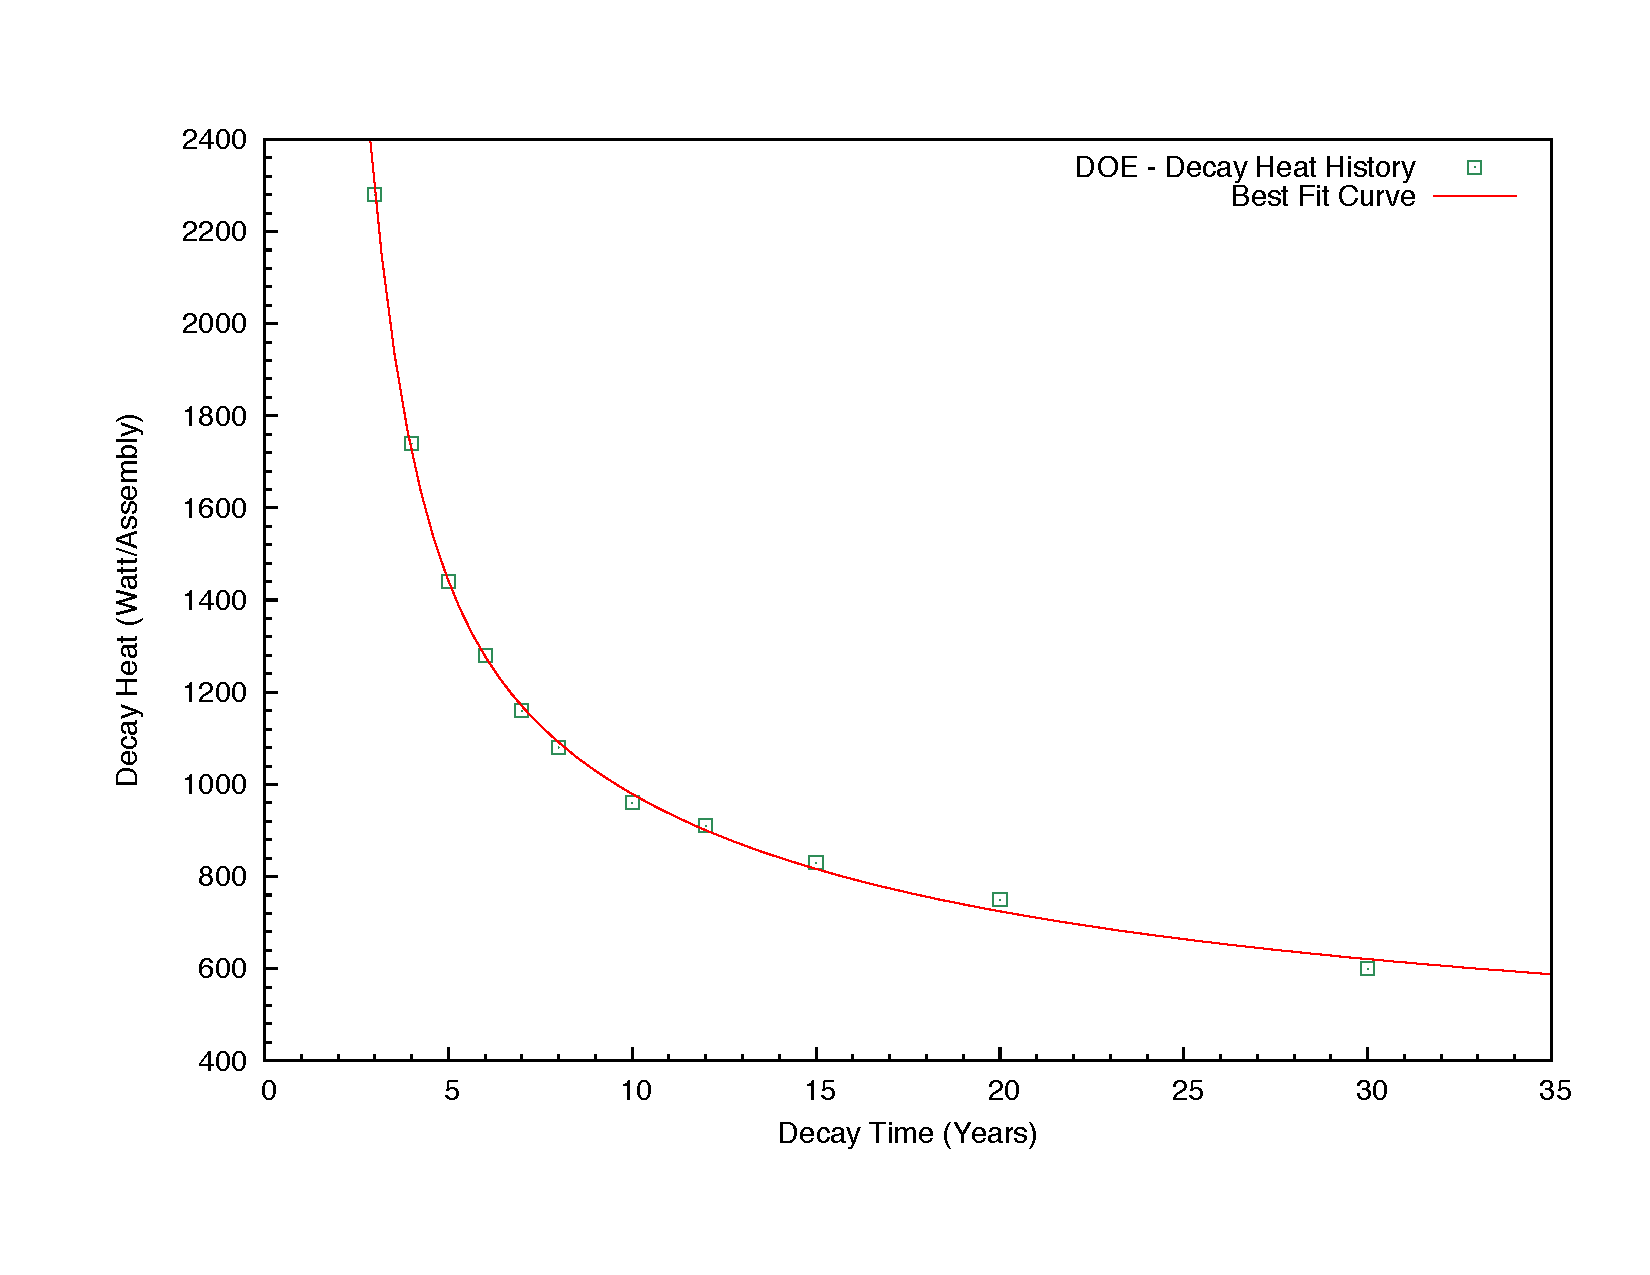
\includegraphics[width=5.5in]{fig_5_1.pdf}
\caption{Decay heat from fission products under storage conditions, from \cite{EPRI1003135}.}
\label{fig:fig_5_1_epri}
\end{figure}


\begin{table*}[!htbp]\centering
\caption{\label{tab1}Simulation properties and constants used.}
\footnotesize
\begin{tabular*}{0.9\textwidth}{@{\extracolsep{\fill}}|c|c|c|c|}\hline
Property&Value&Units&Source\\
\hline
$k(\uo)$&$k(T, x)=\lambda_0(T)\frac{\mbox{arctan}\left(\theta(T, x)\right)}{\theta(T, x)}+5.95\times 10^{-11} T^3$ &$\W\,\m^{-1}\,\K^{-1}$& \cite{ramirez.ea06}\\
&$\begin{array}{r@{\:=\:}l} 
\lambda_0(T)&\left(3.24\times 10^{-2}+2.51\times 10^{-4} T \right)^{-1}\\ 
\theta(T, x) & 3.67 \,\mbox{exp}\left(-4.73\times 10^{-4} T\right)\sqrt{2 x \lambda_0(T)} 
\end{array}$& & \\
\hline
$k(\clad)$&$k(T)=10.98+1.4\times 10^{-2} T-7.44\times 10^{-6} T^2$ &$\W\,\m^{-1}\,\K^{-1}$& \cite{ramirez.ea06}\\
\hline
$r(\uo)$&$r = 0.183$&$\inch$&\cite{roberts75}\\
$r(\clad)$&$r = 0.211$&$\inch$&\cite{roberts75}\\
$l(\uo)$&$l = 0.6$&$\inch$&\cite{roberts75}\\
$T(\mathrm{max})$&$T = 400$&$\C$&\cite{EPRI1015048}\\
\hline
$r(\uo)$&$r_1 = 0.0046482$&$\m$&\cite{roberts75}$^1$\\
$r(\clad)$&$r_2 = 0.0051562$&$\m$&\cite{roberts75}$^1$\\
$r(\mathrm{cask})$&$r_3 = 0.01$&$\m$&\mbox{}$^2$\\
$l(\uo)$&$l = 0.01524$&$\m$&\cite{roberts75}\\
$T(\mathrm{max})$&$T = 673.15$&$\K$&\cite{EPRI1015048}\\
$T_o(\mathrm{ambient})$&$T_o = 313.15$&$\K$&\\
$H_D(t \mathrm{(yr)})$&$H_D = 273.986 + \frac{3113.11}{t^{0.6452}} + 9632.68 \exp(-t)$&$\W / \mathrm{Assy}$&\mbox{}$^3$\\
$k(\uo)$&$k_1= 4.9844$&$\W\,\m^{-1}\,\K^{-1}$&\mbox{}$^4$\\
$k(\clad)$&$k_2= 17.033$&$\W\,\m^{-1}\,\K^{-1}$&\mbox{}$^4$\\
\hline
\end{tabular*}
\begin{minipage}{5.5in}
\hspace{-5pt}\mbox{}$^1$We assumed that both the cladding ID and OD was smaller by the magnitude of
the gap ($0.008\inch$ \cite{roberts75}) or $r_1 = 0.183\inch$ and $r_2 = 0.211 - 0.008 = 0.0203\inch$.
\end{minipage}
\begin{minipage}{5.5in}
\hspace{-5pt}\mbox{}$^2$This is not an important dimension for this calculation, thus an effective radius
of $0.01\m$ is used arbitrarily here.
\end{minipage}
\begin{minipage}{5.5in}
\hspace{-5pt}\mbox{}$^3$Curve fit to data given in Fig.~5--1 in \cite{EPRI1003135}.
\end{minipage}
\begin{minipage}{5.5in}
\hspace{-5pt}\mbox{}$^4$Computed from formula in \cite{ramirez.ea06}, assuming stoichiometric conditions $x = 0$ and
maximum fuel temperature $673.15\K$.
\end{minipage}

\end{table*}

Figure~\ref{fig:fig_5_1_epri} is a recreation of Fig.~5--1 in \cite{EPRI1003135}, that shows fuel decay heat history
vs.\ time in years. This figure is used to create the heat source term in the test problem. Here, we assume there are
$204$ fuel rods per assembly and each rod is $149.7\inch$ in length \cite{roberts75}. We convert the units
to $\W$ per unit length for the 2D test calculation as follows:
%
\begin{equation}
x \frac{\W}{\mathrm{Assy}} \times \frac{\mathrm{Assy}}{204 \, \mathrm{rods}} \times \frac{\mathrm{rod}}{149.7\inch} \times \frac{39.37\inch}{\m}
\label{eq:conversion}
\end{equation}

The properties at the top of Table~\ref{tab1} are from \cite{thermooxy08}. To calculate the energy generation
term, we use the curve fit to Fig.~\ref{fig:fig_5_1_epri}, shown as $H_D$ in
Table~\ref{tab1} to calculate the decay energy generation rate after 8.5 years of
decay \cite{EPRI1003135}, in $\W / \m$. We use \eqref{eq:conversion} for units conversion. This
results in a source term of $1.364\W / \m$ at 8.5 years.  Note that this is the
heat generation in the fuel per meter of rod length. Multiplying by one meter (unit length) this gives the left hand
side of \eqref{eq:energy_balance}, or
%
\begin{equation}
\dot{q}(\pi r^2_1) = 1.364 \W.
\end{equation}
%
This approach assumes no temperature variation vertically in the rod (not a good assumption). Given the radius
of the $\uo$ in the fuel, one may calculate the heat source term at 8.5 years to be 
%
\begin{equation}
\dot{q} = 20095 \W / \m^3.
\end{equation}


\bibliographystyle{plain}
\bibliography{MMbiblio}

\end{document}
